\subsection{Coequalizer of the projections of a fibered square}

Let X and Y be topological spaces, and let f be a continuous map from X to Y. Denote by Z the fibered square \(X \times_{Y} X\) and by \(p_{1}\) , \(p_{2}\) the two projections from Z to X. We denote by W the fibered product \(X \times_{Y} X \times_{Y} X\) ; for every pair \((s, t)\) of elements of \(\{1,2,3\}\) , we denote by \(q_{st}: W \to Z\) the map defined by \(q_{st}(x_{1}, x_{2}, x_{3}) = (x_{s}, x_{t})\) .

Denote by \(\operatorname{Coeg}(f)\) the groupoid \(\operatorname{Coeg}(\varpi(p_{1}),\varpi(p_{2}))\) , the coequalizer of the two morphisms \(\varpi(p_{1})\) , \(\varpi(p_{2})\) from the Poincaré groupoid \(\varpi(Z)\) into the Poincaré groupoid \(\varpi(X)\) . Denote by \(\gamma\colon\varpi(X)\to\operatorname{Coeg}(f)\) the canonical groupoid morphism. Since \(f\circ p_{1}=f\circ p_{2}\) , the groupoid morphisms \(\varpi(f)\circ\varpi(p_{1})\) and \(\varpi(f)\circ\varpi(p_{2})\) from \(\varpi(Z)\) into \(\varpi(Y)\) are equal; there therefore exists a unique groupoid morphism \(\varpi'(f)\colon\operatorname{Coeg}(f)\to\varpi(Y)\) such that \(\varpi'(f)\circ\gamma=\varpi(f)\) .

DEFINITION 1. --- We say that the map f satisfies property (VK) if it is strict, surjective, and if the morphism \(\varpi'(f)\) is an isomorphism.

Example 1. --- This property holds under one of the following hypotheses:

\begin{enumerate}
\def\labelenumi{(\roman{enumi})}
\item
  The spaces X and Y are delaceable, the space \(X \times_{Y} X\) is locally path-connected, the map f is surjective, proper, separated, with locally connected fibers;
\item
  The spaces X and Y are delaceable, the map f is surjective, proper, separated, with finite fibers, the diagonal \(\Delta_{X}\) of \(X \times_{Y} X\) is open and its complement is locally connected;
\item
  The spaces X and Y are delaceable, the map f is surjective, open, and has the path-lifting property;
\item
  Every point of Y has a neighborhood above which there exists a continuous section of the map f.
\end{enumerate}

Indeed, under each of these hypotheses, the map \(f\) is surjective; it is also strict by virtue of I, p. 18, example 2. Finally, the morphism \(\varpi'(f)\) is an isomorphism, whether under hypotheses (i), (ii), or (iii) according to IV, p. 398, th. 1, or under hypothesis (iv) (IV, p. 400, th. 2).

Proposition 5 of II, p. 208 describes the isotropy groups of the groupoid Coeg(f). The aim of this section is to make explicit, when f satisfies property (VK), the description of the Poincaré groups of Y that follows from it by composition with the groupoid isomorphism \(\varpi'(f)\). The following numbers will be devoted to important special cases.

Suppose that the map f satisfies property (VK).

Let us set \(\mathsf{I} = \pi_0(\mathrm{X})\) , \(\mathsf{J} = \pi_0(\mathrm{Z})\) , \(\mathsf{K} = \pi_0(\mathrm{W})\) ; for \(j \in \mathsf{J}\) and \(s \in \{1,2\}\) we set \(i_s(j) = \pi_0(p_s)(j)\) ; for \(k \in \mathsf{K}\) and \(s\) , \(t \in \{1,2,3\}\) we set \(j_{st}(k) = \pi_0(q_{st})(k)\) . Denote by \(\Gamma\) the frame of the pair \((\varpi(p_1), \varpi(p_2))\) of groupoid morphisms from \(\varpi(\mathrm{Z})\) into \(\varpi(\mathrm{X})\) (II, p. 185, def. 3). This is the quiver \((\mathsf{I}, \mathsf{J}, \pi_0(p_1), \pi_0(p_2))\) , for the orbits of the Poincaré groupoid of a topological space are the path-connected components of that space.

Suppose moreover that Y is path-connected and nonempty. By II, p. 200, remark 2, \(\pi_0(\Gamma)\) is then in bijection with the set of orbits of the groupoid Coeg(f); since the map \(f\) satisfies property (VK), the groupoid Coeg(f) is isomorphic to the groupoid \(\varpi(Y)\) . The graph \(\Gamma\) is thus connected and nonempty.

Let us call the van Kampen data of f the data consisting of the following elements:

\begin{enumerate}
\def\labelenumi{(\roman{enumi})}
\item
  for all \(i \in \mathsf{I}\) a point \(\mathsf{a}(i)\) of the path-connected component \(i\) of \(\mathbf{X}\) ;
\item
  for all \(j \in J\) a point \(\mathsf{b}(j) = (\mathsf{b}_{1}(j), \mathsf{b}_{2}(j))\) of the path-connected component j of Z;
\item
  for all \(k \in \mathsf{K}\) a point \(\mathsf{c}(k) = (\mathsf{c}_1(k), \mathsf{c}_2(k), \mathsf{c}_3(k))\) of the path-connected component \(k\) of \(\mathbf{W}\) ;
\item
  for all \(j \in J\) the class \(\beta_{1}(j)\) of a path in X connecting \(\mathsf{b}_{1}(j)\) to \(\mathsf{a}(i_{1}(j))\) and the class \(\beta_{2}(j)\) of a path in X connecting \(\mathsf{b}_{2}(j)\) to \(\mathsf{a}(i_{2}(j))\) ;
\item
  for all \(k \in K\) and for every pair \((s, t)\) equal to \((1, 2)\) , \((2, 3)\) or \((1, 3)\) the class \(\gamma_{st}(k)\) of a path in Z connecting \((\mathsf{c}_{s}(k), \mathsf{c}_{t}(k))\) to \(\mathsf{b}(j_{st}(k))\) ;
\item
  a subquiver \(\mathsf{T}\) of \(\Gamma\) whose associated graph is a maximal tree of the graph \(\widetilde{\Gamma}\) ;
\item
  an element \(i_{0}\) of \(\mathsf{I}\) .
\end{enumerate}

Let us choose a van Kampen datum of \(f\) . Then, \((\mathsf{a},\mathsf{b},\beta_{1},\beta_{2},\mathsf{T},i_{0})\) is a basic datum of the pair \((\varpi(p_{1}),\varpi(p_{2}))\) of groupoid morphisms from \(\varpi(\mathrm{Z})\) on \(\varpi(\mathrm{X})\) (II, p. 192, def. 4). Moreover, the triples

\[
\mathsf {z} = \left(\left(q _ {1 2} (\mathsf {c} (k)), 1\right), \left(q _ {2 3} (\mathsf {c} (k)), 1\right), \left(q _ {1 3} (\mathsf {c} (k)), - 1\right)\right)
\]

and the path classes \((\gamma_{1,2}(k), \gamma_{2,3}(k), \gamma_{1,3}(k))\) , where k ranges over K, define a complementary equipment of the pair \((\varpi(p_{1}), \varpi(p_{2}))\) (II, p. 208, def. 3; II, p. 205, example; II, p. 205, remark). We shall say that the complete equipment of the coequalizer Coeg(f) thus defined is deduced from the van Kampen datum of f that we have chosen.

For every \(j \in J\) , denote by \(\varphi_{j} \colon \pi_{1}(Z, \mathsf{b}(j)) \to \pi_{1}(X, \mathsf{a}(i_{1}(j)))\) and \(\psi_{j} \colon \pi_{1}(Z, \mathsf{b}(j)) \to \pi_{1}(X, \mathsf{a}(i_{2}(j)))\) the group homomorphisms defined by

\[
\varphi_ {j} = \operatorname{Int} (\beta_ {1} (j)) ^ {- 1} \circ (p _ {1}) _ {*}, \quad v \mapsto \beta_ {1} (j) ^ {- 1} ((p _ {1}) _ {*} (v)) \beta_ {1} (j)\tag{1}
\]

\[
\psi_ {j} = \mathrm{Int} (\beta_ {2} (j)) ^ {- 1} \circ (p _ {2}) _ {*}, \quad v \mapsto \beta_ {2} (j) ^ {- 1} ((p _ {2}) _ {*} (v)) \beta_ {2} (j),
\]

for \(v \in \pi_1(\mathbf{Z}, \mathfrak{b}(j))\) . For all \(k \in \mathsf{K}\) and every \(s \in \{1,2,3\}\) , denote by \(\lambda_s(k)\) the loop class at the point \(\mathfrak{a}(i_s(k))\) in X defined by

\[
\lambda_ {1} (k) = \beta_ {1} (j _ {1 3} (k)) ^ {- 1} \cdot ((p _ {1}) _ {*} (\gamma_ {1 3} (k))) ^ {- 1} \cdot ((p _ {1}) _ {*} (\gamma_ {1 2} (k))) \cdot \beta_ {1} (j _ {1 2} (k)),\tag{2}
\]

\[
\lambda_ {2} (k) = \beta_ {2} (j _ {1 2} (k)) ^ {- 1} \cdot ((p _ {2}) _ {*} (\gamma_ {1 2} (k))) ^ {- 1} \cdot ((p _ {1}) _ {*} (\gamma_ {2 3} (k))) \cdot \beta_ {1} (j _ {2 3} (k)),
\]

\[
\lambda_ {3} (k) = \beta_ {2} (j _ {2 3} (k)) ^ {- 1} \cdot ((p _ {2}) _ {*} (\gamma_ {2 3} (k))) ^ {- 1} \cdot ((p _ {2}) _ {*} (\gamma_ {1 3} (k))) \cdot \beta_ {2} (j _ {1 3} (k)).
\]

Denote by \(\tau\) the unique morphism of groupoids from Grp \((\Gamma)\) into \(\varpi(\mathrm{Y})\) such that the map Som \((\tau)\) maps \(i \in \mathsf{I}\) to \(f(\mathsf{a}(i))\) and Fl \((\tau)\) maps \(j \in \mathsf{J}\) to the class of paths \(f_{*}(\beta_{1}(j))^{-1}f_{*}(\beta_{2}(j))\) connecting \(f(\mathsf{a}(i_{1}(j)))\)

\pandocbounded{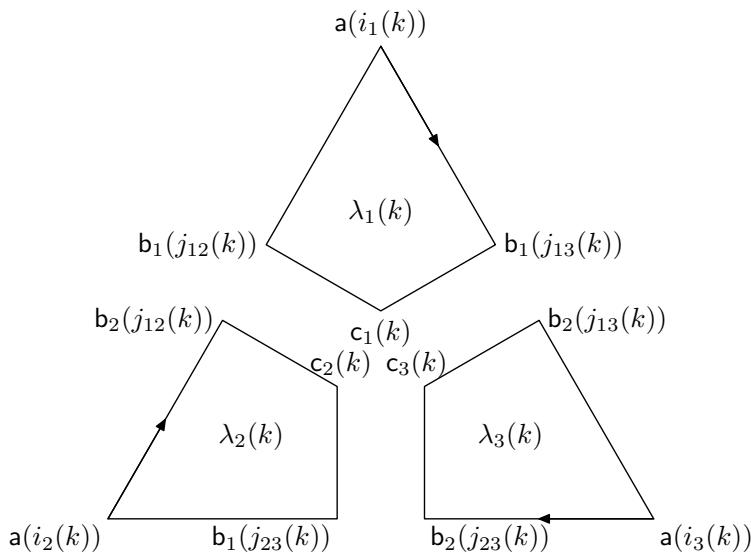
\includegraphics[keepaspectratio]{images/part003_b82e0de6.jpg}}

to \(f(\mathsf{a}(i_2(j)))\) in Y. For \(i \in \mathsf{I}\) , let \(d_i \in \mathrm{Grp}(\Gamma)\) be the class of the unique path without backtracking joining \(i_0\) to \(i\) in the tree \(\widetilde{\mathsf{T}}\) and let us set \(\delta_i = \tau(d_i)\) .

If S is a set, recall that F(S) denotes the free group on S; the image in F(S) of an element \(s \in S\) under the canonical map is denoted {[}s{]}, or even s if there is no possible confusion.

THEOREM 1. --- Suppose that Y is path-connected and that f satisfies property (VK). With the previous notation, there exists a unique group homomorphism

\[
\mathsf {L} \colon \big (\underset {i \in \mathsf {I}} {\ast} \pi_ {1} (\mathrm{X}, \mathsf {a} (i)) \big) \ast \mathrm{F} (\mathrm{J}) \to \pi_ {1} (\mathrm{Y}, f (\mathsf {a} (i _ {0})))
\]

such that

\[
\begin{array}{l l} \mathsf {L} (v) = \delta_ {i} f _ {*} (v) \delta_ {i} ^ {- 1} & \text {for } i\in I \text { and } v\in\pi_{1} (X,a(i)), \\ \mathsf {L} (j) = \delta_ {i _ {1} (j)} \tau (j) \delta_ {i _ {2} (j)} ^ {- 1} & \text {for } j\in J. \end{array}
\]

Moreover, the homomorphism L is surjective and its kernel is the smallest normal subgroup containing the following elements:

\[
\left(\mathrm{R} _ {1}\right) \quad \mathrm{r} _ {1} (j) = j \quad \text {for } j \text { in } \operatorname{Fl} (\mathsf {T});
\]

\[
\left(\mathrm{R} _ {2}\right) \quad \mathfrak {r} _ {2} (j, v) = \varphi_ {j} (v) j \psi_ {j} (v) ^ {- 1} j ^ {- 1} \quad \text {for } j \in \mathsf {J} \text { and } v \in \pi_ {1} (\mathrm{Z}, \mathfrak {b} (j));
\]

\[
\left(\mathrm{R} _ {3}\right) \quad \mathrm{r} _ {3} (k) = \lambda_ {1} (k) j _ {1 2} (k) \lambda_ {2} (k) j _ {2 3} (k) \lambda_ {3} (k) j _ {1 3} (k) ^ {- 1}, \quad \text {for } k \in \mathsf {K}.
\]

The existence and uniqueness of the homomorphism L follow from the universal property of free products and free groups. Moreover, this homomorphism is the composite of the homomorphism \(\varpi'(f)_{\gamma(\mathsf{a}(i_0))}\) deduced from \(\varpi'(f)\) by passing to isotropy groups and to the group homomorphism \(\lambda\) defined by prop. 5 of II, p. 208, taking into account that the chosen van Kampen datum determines a complete equipment of the pair \((\varpi(p_1), \varpi(p_2))\) of groupoid morphisms from \(\varpi(\mathrm{Z})\) into \(\varpi(\mathrm{X})\) . By this proposition, the homomorphism \(\lambda\) has as image the group \(\operatorname{Coeg}(f)_{\gamma(\mathsf{a}(i_0))}\) and its kernel is the smallest normal subgroup containing the elements defined by the relations \((\mathrm{R}_1)\) , \((\mathrm{R}_2)\) and \((\mathrm{R}_3)\) . On the other hand, the groupoid morphism \(\varpi'(f)\) : \(\operatorname{Coeg}(f) \to \varpi(\mathrm{Y})\) is an isomorphism, by definition of property (VK). The theorem is therefore proved.

\subsection{Coverings}

Let Y be a path-connected, nonempty topological space, and let \((\mathrm{A}_{i})_{i\in\mathrm{I}}\) be a covering of Y by nonempty path-connected subsets, indexed by a totally ordered set I. Let \(X=\bigsqcup_{i\in I}A_{i}\) be the sum space of the family \((\mathrm{A}_{i})\) and let \(f:X\to Y\) be the map induced by the family of canonical injections of each \(A_{i}\) in Y. Suppose that the map f satisfies property (VK). This holds in particular in the following two cases:

\begin{enumerate}
\def\labelenumi{(\roman{enumi})}
\item
  the interiors of the sets \(A_{i}\) , for \(i \in I\) cover Y (cf. IV, p. 402, example 2);
\item
  the space Y is delaceable, as are the spaces \(A_{i}\) , for \(i \in I\) , the family \((\mathrm{A}_{i})_{i \in \mathrm{I}}\) is locally finite, the \(A_{i}\) are closed in Y and their pairwise intersections are locally arcwise connected (cf. IV, p. 399, example 1).
\end{enumerate}

Let J' be the set of triples \((i, i', V)\) , where i and \(i'\) are elements of I and where V is a path-connected component of \(A_i \cap A_{i'}\) . If \(j = (i, i', V) \in J'\) we set \(i_1(j) = i\) , \(i_2(j) = i'\) and \(\overline{j} = (i', i, V)\) . Let J be the subset of J' formed by the triples such that \(i < i'\) . We call the frame of the covering the quiver \(\Gamma\) whose set of vertices is I, whose set of arrows is J, and whose origin and target maps are respectively the maps \(j \mapsto i_1(j)\) and \(j \mapsto i_2(j)\) . We shall identify the graph associated with \(\Gamma\) with the graph \(\widetilde{\Gamma}\) whose set of vertices is I, whose set of arrows is \(J \cup \overline{J}\) , whose origin and target maps are the maps \(j \mapsto i_{1}(j)\) and \(j \mapsto i_{2}(j)\) , and whose involution is the map \(j \mapsto \overline{j}\) .

Denote by \(p_1\) and \(p_2\) the projections of the fibered square \(X \times_{Y} X\) onto X; let \(\textsf{Γ}\) be the frame of the pair \((\varpi(p_1), \varpi(p_2))\) of groupoid morphisms from \(\varpi(\mathrm{X} \times_{\mathrm{Y}} \mathrm{X})\) into \(\varpi(\mathrm{X})\) .

Lemma 1. --- The quiver \(\Gamma\) identifies with a subquiver of \(\textsf{Γ}\) ; the quivers \(\Gamma\) and \(\textsf{Γ}\) are connected.

The path-connected components of X are the \(A_{i}\) , for \(i \in I\) . The path-connected components of \(X \times_{Y} X\) are the \((V \times \{i\}) \times_{Y} (V \times \{i'\})\) , for \((i, i', V) \in J'\) . Consequently, the frame \(\textsf{Γ}\) of the pair \((\varpi(p_1), \varpi(p_2))\) is isomorphic to the quiver whose set of vertices is I, whose set of arrows is \(J'\) , the origin and target maps being respectively the maps \(j \mapsto i_1(j)\) and \(j \mapsto i_2(j)\) . The quiver \(\textsf{Γ}\) is connected (IV, p. 406). Moreover, this description identifies \(\Gamma\) with a subquiver of \(\textsf{Γ}\) . Let us also observe that for every arrow j of \(\textsf{Γ}\) , either \(j \in \mathrm{Fl}(\widetilde{\Gamma})\) , or there exists \(i \in I\) such that \(j = (i, i, A_i)\) . It follows that the map \(\pi_0(\Gamma) \to \pi_0(\textsf{Γ})\) deduced from the injection of \(\Gamma\) into \(\textsf{Γ}\) is bijective, so that \(\textsf{Γ}\) is connected.

For every element \(i\) of I, choose a point \(a(i)\) of \(\mathrm{A}_i\) .

For every element \(j = (i, i', \mathrm{V})\) of \(\mathrm{J}\) , choose a point \(b(j)\) on \(\mathrm{V}\) , a path \(\mathrm{B}_1(j)\) connecting \(b(j)\) to \(a(i)\) on \(\mathrm{A}_i\) , and a path \(\mathrm{B}_2(j)\) connecting \(b(j)\) to \(a(i')\) on \(\mathrm{A}_{i'}\) . Let \(j = (i, i', \mathrm{V})\) be an element of \(\overline{\mathrm{J}}\) ; then \(\overline{j} = (i', i, \mathrm{V})\) belongs to \(\mathrm{J}\) , and one sets \(b(\overline{j}) = b(j)\) , \(\mathrm{B}_1(j) = \mathrm{B}_2(\overline{j})\) and \(\mathrm{B}_2(j) = \mathrm{B}_1(\overline{j})\) . For \(j \in \mathrm{J}' \cup \overline{\mathrm{J}'}\) the paths \(\overline{\mathrm{B}_1(j)}\) and \(\mathrm{B}_2(j)\) on \(\mathrm{Y}\) are juxtaposable. Set

\[
\mathrm{B} (j) = \overline {{\mathrm{B} _ {1} (j)}} * \mathrm{B} _ {2} (j).\tag{3}
\]

This is a path joining \(a(i_1(j))\) to \(a(i_2(j))\) in Y; we have the relation \(\mathrm{B}(\overline{j}) = \overline{\mathrm{B}(j)}\) .

For every \(j = (i, i', \mathrm{V}) \in \mathrm{J}'\) , denote by \(p_{j,1} \colon V \to A_i\) and \(p_{j,2} \colon V \to A_{i'}\) the canonical injections; let us also denote by \(\varphi_j \colon \pi_1(\mathrm{V}, b(j)) \to \pi_1(\mathrm{A}_i, a(i))\) and \(\psi_j \colon \pi_1(\mathrm{V}, b(j)) \to \pi_1(\mathrm{A}_{i'}, a(i'))\) the group homomorphisms defined by

\[
\varphi_ {j} (v) = [ \mathrm{B} _ {1} (j) ] ^ {- 1} (p _ {j, 1}) _ {*} (v) [ \mathrm{B} _ {1} (j) ]
\]

and

\[
\psi_ {j} (v) = [ \mathrm{B} _ {2} (j) ] ^ {- 1} (p _ {j, 2}) _ {*} (v) [ \mathrm{B} _ {2} (j) ],
\]

for \(v \in \pi_1(\mathrm{V}, b(j))\) (cf. IV, p. 407).

Fix an element \(i_0\) of I, as well as a subquiver T in the quiver \(\Gamma\) whose associated graph \(\widetilde{T}\) is a maximal tree of the graph \(\widetilde{\Gamma}\) .

For \(i \in I\) , let \((i_0, j_1, i_1, \ldots, j_n, i)\) be the unique path without backtracking joining \(i_0\) to \(i\) in the tree \(\widetilde{T}\) and let us set

\[
\delta (i) = \left[ \mathrm{B} \left(j _ {1}\right) \right] \left[ \mathrm{B} \left(j _ {2}\right) \right] \dots \left[ \mathrm{B} \left(j _ {n}\right) \right];
\]

it is the class of a path joining \(a(i_0)\) to \(a(i)\) in Y. Denote by \(\alpha_i\) the homomorphism from \(\pi_1(\mathrm{A}_i, a(i))\) into \(\pi_1(\mathrm{Y}, a(i))\) deduced from the canonical injection, and let \(\mu_i: \pi_1(\mathrm{A}_i, a(i)) \to \pi_1(\mathrm{Y}, a(i_0))\) be the group homomorphism defined by

\[
\mu_ {i} (v) = \delta (i) \alpha_ {i} (v) \delta (i) ^ {- 1}.
\]

Finally, let \(\mu\colon\mathrm{F}(\mathrm{J})\to\pi_{1}(\mathrm{Y},a(i_{0}))\) the unique group homomorphism such that one has

\[
\mu (j) = \delta (i _ {1} (j)) [ \mathrm{B} (j) ] \delta (i _ {2} (j)) ^ {- 1}
\]

for all \(j \in J\) . There exists a unique group homomorphism

\[
\mathsf {M} \colon \big (\underset {i \in \mathrm{I}} {\ast} \pi_ {1} (\mathrm{A} _ {i}, a (i)) \big) \ast \mathrm{F} (\mathrm{J}) \to \pi_ {1} (\mathrm{Y}, a (i _ {0}))
\]

which coincides with \(\mu_i\) on \(\pi_1(A_i, a(i))\) , for every \(i \in I\) , and with \(\mu\) on \(F(J)\) .

Let K' be the set of quadruples \((i_{1}, i_{2}, i_{3}, \mathrm{U})\) , where \(i_{1}, i_{2}, i_{3}\) are elements of I and where U is a path-connected component of \(A_{i_{1}} \cap A_{i_{2}} \cap A_{i_{3}}\) . For every element \(k = (i_{1}, i_{2}, i_{3}, \mathrm{U})\) of \(K'\) and every pair \((s, t)\) of elements of \(\{1, 2, 3\}\) we set \(j_{st}(k) = (i_{s}, i_{t}, \mathrm{V})\) , where V is the path-connected component of \(A_{i_{s}} \cap A_{i_{t}}\) that contains U; this is an element of \(J'\) .

Let K be the subset of \(K'\) formed by the quadruples \((i_{1}, i_{2}, i_{3}, \mathrm{U})\) such that \(i_{1} < i_{2} < i_{3}\) . For every element \(k = (i_{1}, i_{2}, i_{3}, \mathrm{U})\) of K, choose a point \(c(k)\) of U, as well as paths \(\mathrm{C}_{12}(k)\) , \(\mathrm{C}_{23}(k)\) and \(\mathrm{C}_{13}(k)\) such that \(\mathrm{C}_{st}(k)\) connects \(c(k)\) to \(b(j_{st}(k))\) in \(A_{i_{s}} \cap A_{i_{t}}\) for \(s, t \in \{1, 2, 3\}\) with s \textless{} t.

Let us then set, for \(k \in \mathbf{K}\) ,

\[
\mathrm{L} _ {1} (k) = \overline {{\mathrm{B} _ {1} (j _ {1 3} (k))}} * \overline {{\mathrm{C} _ {1 3} (k)}} * \mathrm{C} _ {1 2} (k) * \mathrm{B} _ {1} (j _ {1 2} (k)),\tag{4}
\]

\[
\mathrm{L} _ {2} (k) = \overline {{\mathrm{B} _ {2} (j _ {1 2} (k))}} * \overline {{\mathrm{C} _ {1 2} (k)}} * \mathrm{C} _ {2 3} (k) * \mathrm{B} _ {1} (j _ {2 3} (k)),
\]

\[
\mathrm{L} _ {3} (k) = \overline {{\mathrm{B} _ {2} (j _ {2 3} (k))}} * \overline {{\mathrm{C} _ {2 3} (k)}} * \mathrm{C} _ {1 3} (k) * \mathrm{B} _ {2} (j _ {1 3} (k)).
\]

For \(s \in \{1,2,3\}\) , denote by \(\lambda_s(k)\) the class in \(\pi_1(\mathrm{A}_{i_s}, a(i_s))\) of the loop \(\mathrm{L}_s(k)\) .

PROPOSITION 1. --- Let Y be a path-connected topological space and let \((\mathrm{A}_{i})_{i\in\mathrm{I}}\) be a covering of Y by nonempty, path-connected subsets, indexed by a totally ordered set I. Suppose that the canonical map from the sum space of the family \((\mathrm{A}_{i})_{i\in\mathrm{I}}\) into Y satisfies property (VK). Then, the homomorphism M introduced above is surjective and its kernel is the smallest normal subgroup containing the following elements:

\[
\begin{array}{l} \text {(R$_ {1}$)} r _ {1} (j) = j \qquad \text {for } j \text { in } \operatorname{Fl}(\mathsf {T}); \\ \text {(R$_ {2}$)} r _ {2} (j, v) = \varphi_ {j} (v) j \psi_ {j} (v) ^ {- 1} j ^ {- 1} \\ \qquad \qquad \qquad \qquad \qquad \qquad \qquad \qquad \qquad \text {for } j = (i,i^{\prime} ,V)\in \mathsf {J} \text { and } v\in\pi_{1} (V,b(j)); \\ \text {(R$_ {3}$)} r _ {3} (k) = \lambda_ {1} (k) j _ {1 2} (k) \lambda_ {2} (k) j _ {2 3} (k) \lambda_ {3} (k) j _ {1 3} (k) ^ {- 1} \\ \qquad \qquad \qquad \qquad \qquad \qquad \qquad \qquad \text {for } k\in \mathsf {K}. \end{array}
\]

Let X be the topological space that is the sum of the family \((\mathrm{A}_{i})_{i\in\mathrm{I}}\) and let \(f\colon X\to Y\) be the map induced by the family of canonical injections of each \(A_{i}\) in Y. The map f satisfies property (VK) by hypothesis; we shall therefore apply to it th. 1 of no. 1. We thus resume the notation of that section and begin by defining a van Kampen datum for the map f.

The path-connected components of X are the sets \(X_{i} = A_{i} \times \{i\}\) for \(i \in I\) . One thus identifies \(\pi_{0}(X)\) with the set I. For every \(i \in I\) , denote by \(\mathfrak{a}(i)\) the point \((a(i), i)\) of \(X_{i}\) .

Let us set \(Z = X \times_{Y} X\) . The path-connected components of \(Z\) are the sets \(Z_j = (V \times \{i\}) \times_{Y} (V \times \{i'\})\) , where \(j = (i, i', V)\) runs through \(J'\) . One thus identifies \(\pi_0(Z)\) with the set \(J'\) . Let \(J_0\) be the set of elements of \(J\) of the form \((i, i, A_i)\) , so that the family \((J_0, J, \overline{J})\) is a partition of \(J'\) . For \(i \in I\) and \(j = (i, i, A_i) \in J_0\) , set \(b(j) = (a(i), a(i))\) and take for \(\beta_1(j)\) and \(\beta_2(j)\) the class of the constant path at \(a(i)\) . For \(j = (i, i', V) \in J \cup \overline{J}\) , denote by \(b(j)\) the point \(((b(j), i), (b(j), i'))\) of \(Z_j\) and denote by \(\beta_1(j)\) and \(\beta_2(j)\) the classes of paths \(t \mapsto (B_1(j)(t), i)\) and \(t \mapsto (B_2(j)(t), i')\) on \(X\) .

Let us set \(W = X \times_{Y} X \times_{Y} X\) . The path-connected components of W are the sets \(W_k = (U \times \{i_1\}) \times_{Y} (U \times \{i_2\}) \times_{Y} (U \times \{i_3\})\) , where \(k = (i_1, i_2, i_3, U)\) runs through \(K'\) . One thus identifies \(\pi_0(W)\) with the set \(K'\) .

Denote by \(K_{0}\) the set of elements of \(K'\) of the form \(k = (i, i, i, A_{i})\) , for \(i \in I\) . For such an element \(k \in K_{0}\) we set \(\mathsf{c}(k) = (\mathsf{a}(i), \mathsf{a}(i), \mathsf{a}(i))\) and one chooses for \(\gamma_{st}(k)\) the class of the constant path at \((\mathsf{a}(i), \mathsf{a}(i))\) .

Denote by \(K_{1}\) the set of elements of \(K'\) of the form \(k = (i_{1}, i_{2}, i_{3}, V)\) for which the set \(\{i_{1}, i_{2}, i_{3}\}\) has two elements. Let k be an element of \(K'\) of the form \((i, i, i', V)\) , such that \(j = (i, i', V)\) belongs to \(J \cup \overline{J}\) . We then set

\[
\mathsf {c} (k) = ((b (j), i), (b (j), i), (b (j), i ^ {\prime})), \quad \gamma_ {1 2} (k) = (\beta_ {1} (j), \beta_ {1} (j))
\]

and we take for \(\gamma_{13}(k)\) and \(\gamma_{23}(k)\) the class of the constant path at \(\mathsf{b}(j)\) . One defines analogously \(c(k)\) , \(\gamma_{12}(k)\) , \(\gamma_{13}(k)\) , \(\gamma_{23}(k)\) for every element \(k\) of \(\mathrm{K}'\) .

For every element \(k = (i_{1}, i_{2}, i_{3}, \mathrm{U})\) of K, set

\[
\mathsf {c} (k) = ((c (k), i _ {1}), (c (k), i _ {2}), (c (k), i _ {3})) ;
\]

for every pair \((s,t)\) of distinct elements of \(\{1,2,3\}\) , take for \(\gamma_{st}(k)\) the image under the map \(x\mapsto((x,s),(x,t))\) of the class of the path \(\mathrm{C}_{st}(k)\) in \(\mathrm{A}_{i_{s}(k)}\cap\mathrm{A}_{i_{t}(k)}\) .

For every point \(x = (x_1, x_2, x_3)\) of \(X \times_Y X \times_Y X\) and any permutation \(\sigma \in \mathfrak{S}_3\) , set \(\sigma(x) = (x_{\sigma^{-1}(1)}, x_{\sigma^{-1}(2)}, x_{\sigma^{-1}(3)})\) . One thus defines an action of the group \(\mathfrak{S}_3\) on W. For every \(k = (i_1, i_2, i_3, U) \in K'\) and any permutation \(\sigma \in \mathfrak{S}_3\) , set similarly \(\sigma(k) = (i_{\sigma^{-1}(1)}, i_{\sigma^{-1}(2)}, i_{\sigma^{-1}(3)}, U)\) ; we have

\[
\sigma \left(\mathrm{W} _ {k}\right) = \left(\mathrm{U} \times \left\{i _ {\sigma^ {- 1} (1)} \right\}\right) \times_ {\mathrm{Y}} \left(\mathrm{U} \times \left\{i _ {\sigma^ {- 1} (2)} \right\}\right) \times_ {\mathrm{Y}} \left(\mathrm{U} \times \left\{i _ {\sigma^ {- 1} (3)} \right\}\right) = \mathrm{W} _ {\sigma (k)}.
\]

Let \(k = (i_1, i_2, i_3, \mathrm{U})\) be an element of \(\mathrm{K}'\) such that \(i_1, i_2, i_3\) are pairwise distinct. There exists a unique permutation \(\sigma \in \mathfrak{S}_3\) such that \(i_{\sigma^{-1}(1)} < i_{\sigma^{-1}(2)} < i_{\sigma^{-1}(3)}\) , such that \(\sigma(k) = (i_{\sigma^{-1}(1)}, i_{\sigma^{-1}(2)}, i_{\sigma^{-1}(3)}, \mathrm{U})\) belongs to \(\mathrm{K}\) . For \(s \in \{1, 2, 3\}\) , one then sets \(c_s(k) = c_{\sigma(s)}(\sigma(k))\) and \(c(k) = (c_1(k), c_2(k), c_3(k))\) , such that \(c(k) = \sigma^{-1}(c(\sigma(k)))\) . For \((s, t) \in \{(1, 2), (1, 3), (2, 3)\}\) , one defines \(\mathrm{C}_{st}(k) = \mathrm{C}_{\sigma^{-1}(s)\sigma^{-1}(t)}(\sigma(k))\) ; this is a path that connects \(c(k)\) to \(b(j_{\sigma(s)\sigma(t)}(\sigma(k))) = b(j_{st}(k))\) .

Denote by \(g\) the quiver morphism from \(\Gamma\) into \(\textsf{Γ}\) which, to a vertex \(i \in I\) of \(\Gamma\) , associates the vertex \(X_i = A_i \times \{i\}\) of \(\textsf{Γ}\) and, to an arrow \(j = (i, i', V) \in J'\) of \(\Gamma\) , associates the arrow \(Z_j = (V \times \{i\}) \times_Y(V \times \{i'\})\) of \(\textsf{Γ}\) . The map Som( \(g\) ) is bijective; the map Fl( \(g\) ) is injective and the graph \(\Gamma\) is connected (IV, p. 410, lemma 1) and the image under \(g\) of the subquiver T is a subquiver \(\mathsf{T}\) of \(\textsf{Γ}\) whose associated graph is a maximal tree of the graph \(\widetilde{\textsf{Γ}}\) .

The points \(\mathsf{a}(i)\) , for \(i \in I\) , the point \(\mathsf{b}(j)\) , for \(j \in J'\) , the points \(\mathsf{c}(k)\) , for \(k \in K'\) , the path classes \(\beta_{1}(j)\) and \(\beta_{2}(j)\) , for \(j \in J'\) , the path classes \(\gamma_{st}(k)\) , for \(k \in \mathrm{K}'\) , the subquiver \(g(\mathrm{T})\) of \(\textsf{Γ}\) and the element \(i_0\) of I define a van Kampen datum of \(f\) .

Denote by \(\rho\) the unique group homomorphism

\[
\rho \colon \big (\underset {i \in \mathrm{I}} {*} \pi_ {1} (\mathrm{X}, \mathsf {a} (i)) \big) * \mathrm{F} (\mathrm{J} ^ {\prime}) \to \big (\underset {i \in \mathrm{I}} {*} \pi_ {1} (\mathrm{A} _ {i}, a (i)) \big) * \mathrm{F} (\mathrm{J})
\]

which induces the isomorphism of \(\pi_1(\mathrm{X},\mathsf{a}(i))\) onto \(\pi_1(\mathrm{A}_i,a(i))\) deduced from the identification of \(\mathrm{A}_i\times \{i\}\) and \(\mathrm{A}_i\) , for every \(i\in \mathrm{I}\) , and such that one has

\[
\begin{array}{l l} \rho (j) = 1 & \text {for } j \in \mathrm{J} _ {0} \\ \rho (j) = j, \quad \rho (\overline {{j}}) = j ^ {- 1} & \text {for } j \in \mathrm{J}. \end{array}
\]

Let L be the group homomorphism defined in th. 1 of IV, p. 408. For \(j = (i, i, \mathrm{A}_i) \in \mathrm{J}_0\) , we have \(\mathsf{L}(j) = 1 = \mathsf{M} \circ \rho(j)\) . Let \(j = (i, i', \mathrm{V})\) an element of J; we have \(\mathsf{L}(j) = (\mathsf{M} \circ \rho)(j)\) by definition. Finally, if \(j = (i, i', \mathrm{V})\) is an element of \(\overline{\mathbf{J}}\) , \(\overline{j} \in \mathbf{J}\) and one verifies that

\[
\mathsf {L} (j) = \mathsf {L} (\overline {{j}}) ^ {- 1} = \mathsf {M} (\rho (\overline {{j}})) ^ {- 1} = \mathsf {M} (\rho (j)).
\]

Consequently, we have M ∘ ρ = L.

The homomorphism L is surjective (loc. cit.), hence the homomorphism M is also surjective. Since the homomorphism \(\rho\) is surjective, the kernel of M is the smallest normal subgroup of \(\left(\ast\pi_{1}(\mathrm{A}_{i},a(i))\right)*\mathrm{F}(\mathrm{J})\) which contains the images under \(\rho\) of the elements defined by the relations \((\mathrm{R}_{1})\) , \((\mathrm{R}_{2})\) , \((\mathrm{R}_{3})\) of Theorem 1 (IV, p. 408). The proof will be complete once we have verified that these images are, besides the elements defined by the relations \((\mathrm{R}_{1})\) , \((\mathrm{R}_{2})\) , \((\mathrm{R}_{3})\) of prop. 1, the elements conjugate to them, or conjugate to their inverses, as well as the identity element.

Elements R \(_{1}\) --- An arrow of the oriented tree T is of the form Z \(_{j}\) , with \(j = (i, i', V) \in J\) ; its image is the element \(j\) of F(J).

Elements R₂. --- Let \(j = (i, i', \mathrm{V}) \in \mathrm{J}'\) . If \(i = i'\) , we have \(\rho(\mathsf{r}_2(j, v)) = 1\) for all \(v \in \pi_1(\mathrm{A}_i, \mathsf{a}(i))\) . If \(j \in J\) the image of \(\mathsf{r}_2(j, v)\) is the element \(r_2(j, v) = \varphi_j(v) j \psi_j(v)^{-1} j^{-1}\) , for every \(v \in \pi_1(\mathrm{Z}, \mathsf{b}(j))\) . In the remaining case, we have \(\overline{j} \in J\) and the equality

\[
\begin{array}{r l} & {\rho (\mathtt {r} _ {2} (j, v)) = \rho (\varphi_ {j} (v) j \psi_ {j} (v) ^ {- 1} j ^ {- 1})} \\ & {\qquad = [ \mathrm{B} _ {1} (j) ] ^ {- 1} v [ \mathrm{B} _ {1} (j) ] \rho (j) [ \mathrm{B} _ {2} (j) ] ^ {- 1} v ^ {- 1} [ \mathrm{B} _ {2} (j) ] \rho (j) ^ {- 1}} \\ & {\qquad = [ \mathrm{B} _ {2} (\bar {j}) ] ^ {- 1} v [ \mathrm{B} _ {2} (\bar {j}) ] \bar {j} ^ {- 1} [ \mathrm{B} _ {1} (\bar {j}) ] ^ {- 1} v ^ {- 1} [ \mathrm{B} _ {1} (\bar {j}) ] \bar {j}} \end{array}
\]

entails that \(\rho(\mathsf{r}_2(j,v))\) is conjugate to \(\rho(\mathsf{r}_2(\overline{j},v^{-1}))\) .

Elements R₃. — Let \(k = (i_{1}, i_{2}, i_{3}, \mathrm{U})\) be an element of K'.

If \(k \in \mathrm{K}_0\) , \(i_1 = i_2 = i_3\) , \(\lambda_s(k)\) is the class of the trivial path for all \(s \in \{1,2,3\}\) , \(j_{st}(k) \in \mathrm{J}_0\) for every pair \((s,t) \in \{(1,2),(1,3),(2,3)\}\) . Then, \(\rho(\mathsf{r}_3(k))\) is the identity element.

Suppose \(k\in \mathrm{K}_1\) . If \(i_1 = i_2\) then \(j = (i_{1},i_{3},\mathrm{U})\in \mathrm{J}\cup \overline{\mathrm{J}}\) and one has

\[
\mathsf {r} _ {3} (k) = \beta_ {1} (j) ^ {- 1} j _ {1 2} \beta_ {1} (j) j _ {2 3} \beta_ {2} (j) ^ {- 1} \beta_ {2} (j) j _ {1 3} ^ {- 1}
\]

whose image under \(\rho\) is the identity element. The other cases are handled similarly.

Suppose that \(i_{1}, i_{2}, i_{3}\) are pairwise distinct. If \(i_{1} < i_{2} < i_{3}\) , \(k \in \mathbf{K}\) and the image of \(\rho(\mathsf{r}_{3}(k))\) is the element \(r_{3}(k)\) .

Let \(\sigma \in \mathfrak{S}_3\) be the permutation that maps 1 to 2 and 2 to 3. We have

\[
\begin{array}{r l} \lambda_ {1} (\sigma (k)) & = \beta_ {1} (j _ {1 3} (\sigma (k))) ^ {- 1} \cdot p _ {1, *} (\gamma_ {1 3} (\sigma (k))) ^ {- 1} \cdot \\ & \qquad \cdot p _ {1, *} (\gamma_ {1 2} (\sigma (k))) \cdot \beta_ {1} (j _ {1 2} (\sigma (k))) \\ & = \beta_ {1} (j _ {3 2} (k)) ^ {- 1} \cdot p _ {1, *} (\gamma_ {3 2} (k)) ^ {- 1} \cdot p _ {1, *} (\gamma_ {3 1} (k)) \cdot \beta_ {1} (j _ {3 1} (k)) \\ & = \beta_ {2} (j _ {2 3} (k)) ^ {- 1} \cdot p _ {2, *} (\gamma_ {2, 3} (k)) ^ {- 1} \cdot p _ {2, *} (\gamma_ {1 3} (k)) \cdot \beta_ {2} (j _ {1 3} (k)) \\ & = \lambda_ {3} (k). \end{array}
\]

We check similarly that we have \(\lambda_2(\sigma(k)) = \lambda_1(k)\) and \(\lambda_3(\sigma(k)) = \lambda_2(k)\) . Consequently,

\[
\begin{array}{r l} & {\rho (\mathsf {r} _ {3} (\sigma (k))) = \lambda_ {1} (\sigma (k)) \rho (j _ {1 2} (\sigma (k))) \lambda_ {2} (\sigma (k)) \cdot} \\ & {\qquad \cdot \rho (j _ {2 3} (\sigma (k))) \lambda_ {3} (\sigma (k)) \rho (j _ {1 3} (\sigma (k))) ^ {- 1}} \\ & {\qquad = \lambda_ {3} (k) \rho (j _ {3 1} (k)) \lambda_ {1} (k) \rho (j _ {1 2} (k)) \lambda_ {2} (k) \rho (j _ {3 2} (k)) ^ {- 1}} \\ & {\qquad = \lambda_ {3} (k) j _ {1 3} (k) ^ {- 1} \lambda_ {1} (k) j _ {1 2} (k) \lambda_ {2} (k) j _ {2 3} (k),} \end{array}
\]

which proves that \(\rho(\mathsf{r}_3(\sigma(k)))\) is conjugate to

\[
\lambda_ {1} (k) j _ {1 2} (k) \lambda_ {2} (k) j _ {2 3} (k) \lambda_ {3} (k) j _ {1 3} (k) ^ {- 1} = \rho (\mathsf {r} _ {3} (k)).
\]

Let \(\tau \in \mathfrak{S}_3\) be the transposition with support \(\{1,2\}\) . We have

\[
\lambda_ {1} (\tau (k)) = \lambda_ {2} (k) ^ {- 1}, \quad \lambda_ {2} (\tau (k)) = \lambda_ {1} (k) ^ {- 1} \quad \text {and} \quad \lambda_ {3} (\tau (k)) = \lambda_ {3} (k) ^ {- 1}.
\]

The equalities

\[
\begin{array}{c} \rho (\mathsf {r} _ {3} (\tau (k))) = \lambda_ {2} (k) ^ {- 1} \rho (j _ {2 1} (k)) \lambda_ {1} (k) ^ {- 1} \rho (j _ {1 3} (k)) \lambda_ {3} (k) ^ {- 1} \rho (j _ {2 3} (k)) ^ {- 1} \\ = \big (\rho (j _ {2 3} (k)) \lambda_ {3} (k) \rho (j _ {1 3} (k)) ^ {- 1} \lambda_ {1} (k) \rho (j _ {1 2} (k)) \lambda_ {2} (k) \big) ^ {- 1} \end{array}
\]

show that \(\rho(\mathsf{r}_3(\tau(k)))\) is conjugate to the inverse of

\[
\lambda_ {1} (k) \rho (j _ {1 2} (k)) ^ {- 1} \lambda_ {2} (k) \rho (j _ {2 3} (k)) \lambda_ {3} (k) \rho (j _ {1 3} (k)) ^ {- 1} = \rho (\mathsf {r} _ {3} (k)).
\]

Since the group \(\mathfrak{S}_3\) is generated by the permutations \(\tau\) and \(\sigma\) , it follows that, for every \(k \in \mathrm{K}\) and every \(\sigma \in \mathfrak{S}_3\) , \(\rho(\mathsf{r}_3(\sigma(k)))\) is conjugate to \(\rho(\mathsf{r}_3(k))\) or to its inverse.

Proposition 1 is thus proved.

COROLLARY 1. --- Under the hypotheses of Proposition 1, suppose further that, for every \(i \in I\) the image of the homomorphism from \(\pi_1(A_i, a(i))\) into \(\pi_1(Y, a(i))\) deduced from the canonical injection of \(A_i\) in Y is trivial. The homomorphism \(M': F(J) \to \pi_1(Y, a(i_0))\) deduced from M by restriction is then surjective and its kernel is the smallest normal subgroup containing the elements \(j \in Fl(T)\) and the elements \(j_{12}(k) j_{23}(k) j_{13}(k)^{-1}\) for \(k \in K\) .

Let \(\pi\colon (*_{i\in\mathrm{I}}\pi_1(\mathrm{A}_i,a(i)))*\mathrm{F}(\mathrm{J})\to\mathrm{F}(\mathrm{J})\) be the unique homomorphism that induces the trivial homomorphism on each \(\pi_1(\mathrm{A}_i,a(i))\) and the identity on \(\mathrm{F}(\mathrm{J})\) ; it is surjective. Let \(i\in\mathrm{I}\) . The definition of \(\mathsf{M}\) and the hypothesis that the image of the homomorphism from \(\pi_1(\mathrm{A}_i,a(i))\) into \(\pi_1(\mathrm{Y},a(i))\) deduced from the canonical injection is trivial imply that, for every \(v\in\pi_1(\mathrm{A}_i,a(i))\) , \(\mathsf{M}(v)\) is the identity element of \(\pi_1(\mathrm{Y},a(i_0))\) . We therefore have \(\mathsf{M}=\mathsf{M}'\circ\pi\) . Consequently, the homomorphism \(\mathsf{M}'\) is surjective and its kernel is the smallest normal subgroup containing the images under \(\pi\) of the elements \(r_1(j)\) , \(r_2(j,v)\) and \(r_3(k)\) defined in Prop. 1. For \(j\in\mathrm{Fl}(\mathrm{T})\) , we have \(\pi(r_1(j))=j\) . For all \(j\in\mathrm{J}\) and every \(v\in\pi_1(\mathrm{V},b(j))\) , we have \(\pi(r_2(j,v))=e\) . Finally, for every \(k=(i_1,i_2,i_3,\mathrm{U})\in\mathrm{K}\) and every \(s\in\{1,2,3\}\) , \(\lambda_s(k)\) is the class of a loop in \(\mathrm{A}_{i_s}\) ; one therefore has \(\pi(\lambda_s(k))=e\) , so that \(\pi(r_3(k))=j_{12}(k)j_{23}(k)j_{13}(k)^{-1}\) . The corollary follows from this.

COROLLARY 2. --- Under the hypotheses of Proposition 1, suppose further that for every \(i \in I\) , the group \(\pi_1(A_i, a(i))\) is reduced to the identity element and that, for every triple \((i_1, i_2, i_3)\) of pairwise distinct elements of I, the set \(A_{i_1} \cap A_{i_2} \cap A_{i_3}\) is empty. The homomorphism \(\mathsf{M}''\colon \mathrm{F}(\mathrm{J} - \mathrm{Fl}(\mathrm{T})) \to \pi_1(\mathrm{Y}, a(i_0))\) deduced from \(\mathsf{M}\) by restriction is then an isomorphism.

Let \(\pi'\colon\mathrm{F}(\mathrm{J})\to\mathrm{F}(\mathrm{J}-\mathrm{Fl}(\mathrm{T}))\) be the homomorphism which maps \([j]\) onto \([j]\) if \(j\in\mathrm{J}-\mathrm{Fl}(\mathrm{T})\) and which maps \([j]\) to the identity element if \(j\in\mathrm{Fl}(\mathrm{T})\) ; it is surjective and we have \(\mathsf{M}''\circ\pi'= \mathsf{M}'\) , where \(\mathsf{M}'\) is the surjective homomorphism defined in Corollary 1. It follows that \(\mathsf{M}''\) is surjective and its kernel is the smallest normal subgroup of \(\mathrm{F}(\mathrm{J}-\mathrm{Fl}(\mathrm{T}))\) which contains the images under \(\pi'\) of the elements described in loc. cit. Now, by construction, \(\pi'(j) = e\) if \(j \in \mathrm{Fl}(T)\) and the set K is empty, by hypothesis. The homomorphism \(M''\) is therefore an isomorphism.

Examples. --- 1) For the case of a covering formed by two sets, see No. 3.

\begin{enumerate}
\def\labelenumi{\arabic{enumi})}
\setcounter{enumi}{1}
\tightlist
\item
  Let G be a graph (II, p. 155, Definition 1); denote by S the set of vertices of G, by A the set of its oriented edges, and by o and t the origin and terminus maps from A to S; for every oriented edge \(a \in A\) , write \(\overline{a}\) the opposite oriented edge. Endow the sets S and A with the discrete topology; let X be the sum space of the space S and the space I × A, and let ∼ be the finest equivalence relation on X for which \((u, a) \sim (1 - u, \overline{a})\) , \((0, a) \sim o(a)\) and \((1, a) \sim t(a)\) for all \(u \in I\) and every oriented edge \(a \in A\) . The quotient space \(|G| = X / \sim\) is called the geometric realization of the graph G. We denote by p the canonical projection of X onto \(|G|\) .
\end{enumerate}

Let us prove that \(|\mathbf{G}|\) is locally contractible. Let \(s \in S\) . Denote by \(\mathrm{X}_s\) the union of \(\{s\}\) and the subsets \([0,1[ \times \{a\}\) for \(a \in o^{-1}(s)\) and the subsets \(]0,1] \times \{a\}\) for \(a \in t^{-1}(s)\) . Let \(\mathrm{U}_s\) be the image of \(\mathrm{X}_s\) in \(|\mathbf{G}|\) ; it is an open neighborhood of \(p(s)\) in \(|\mathbf{G}|\) since \(\mathrm{X}_s\) is a saturated open neighborhood of \(s\) in \(X\) . Let \(f\) be the map from \(\mathrm{X}_s \times \mathbf{I}\) into \(\mathrm{X}_s\) defined, for \(u, v \in \mathbf{I}\) and \(a \in A\) by the relations

\[
\begin{array}{c} f (s, v) = s \\ f ((u, a), v) = \left\{ \begin{array}{l l} ((1 - v) u, a) & \text {if } 0 \leqslant u <   1 \text {and } o (a) = s, \\ (1 - (1 - v) (1 - u), a) & \text {if } 0 <   u \leqslant 1 \text {and } t (a) = s. \end{array} \right. \end{array}
\]

It is continuous and compatible with the equivalence relation ∼. It therefore defines, by passing to the quotient, a map \(\varphi_{s}\colon U_{s}\times I\to U_{s}\) which is continuous, since I is locally compact (I, p. 19, prop. 10). It is a strong contraction of \(U_{s}\) onto \(p(s)\) (III, p. 237, def. 6).

Let moreover \(x = (\tau, a) \in ]0, 1[ \times \mathrm{A}\) . Denote by \(\mathrm{X}_x = ]0, 1[ \times \{a, \overline{a}\}\) and let \(\mathrm{U}_x\) be its image in \(|\mathbf{G}|\) under \(p\) ; it is a neighborhood of \(p(x)\) in \(|\mathbf{G}|\) , homeomorphic to \(]0, 1[\) . The map from \(\mathrm{X}_x \times \mathbf{I}\) into \(\mathrm{X}_x\) given by \(((u, a), v) \mapsto ((1 - v)u + v\tau, a)\) and \(((u, \overline{a}), t) \mapsto ((1 - v)u + v(1 - \tau), \overline{a})\) is continuous. By passing to the quotient it defines a map \(\varphi_x: \mathrm{U}_x \times \mathbf{I} \to \mathrm{U}_x\) which is continuous (loc. cit.) and is a strong contraction at \(x\) .

Every point of \(|\mathbf{G}|\) is the image of a point \(s \in \mathbf{S}\) or of a point of \(\mathbf{I} \times \mathbf{A}\) of the form \((\tau, a)\) where \(0 < \tau < 1\) . It follows that every point of \(|\mathbf{G}|\) has a contractible neighborhood at this point. In other words, \(|\mathbf{G}|\) is locally contractible and, in particular, simply connected (IV, p. 346, prop. 5).

Choose a total order on S and consider the open covering \((\mathrm{U}_{s})_{s\in\mathrm{S}}\) of \(|G|\) . Let s and \(s'\) be distinct elements of S. The intersection \(U_{s}\cap U_{s'}\) is the union of the \(p([0,1[,a)\) where a ranges over the set of oriented edges of G whose endpoints are s and \(s'\) . Consequently, the nerve of the covering \((\mathrm{U}_{s})_{s\in\mathrm{S}}\) is identified with the quiver G. Moreover, for every \(s\in S\) , \(U_{s}\) is contractible at s, hence \(\pi_{1}(\mathrm{U}_{s},p(s))\) is reduced to the identity element. It then follows from cor. 2 of IV, p. 416 that for every \(s\in S\) , \(\pi_{1}(|\mathrm{G}|,p(s))\) is a free group (Nielsen-Schreier theorem).

COROLLARY 3. --- Under the hypotheses of prop. 1, suppose moreover that the frame of the covering (A \(_{i}\) ) \(_{i\in I}\) is an oriented tree. The homomorphism N: * \(_{i\in I} \pi_{1}(A_{i},a(i)) \to \pi_{1}(Y,a(i_{0}))\) deduced from M by restriction is then surjective; its kernel is the smallest distinguished subgroup of * \(_{i\in I} \pi_{1}(A_{i},a(i))\) which contains the elements \(\varphi_{j}(v)\psi_{j}(v)^{-1}\) , for every \(j = (i_{1},i_{2},V) \in J\) and every \(v \in \pi_{1}(V,b(j))\) .

If the path-connected components of the intersections \(A_{i} \cap A_{i'}\) , for \(i \neq i'\) are moreover simply connected by arcs, the homomorphism N is then an isomorphism.

Under the hypotheses of the corollary, the graph associated with the quiver \(\Gamma\) is a tree, whence \(T = \Gamma\) . It follows that the image of the group \(F(J)\) under the homomorphism \(M\) is reduced to the identity element.

Let

\[
\rho \colon \big (\underset {i \in \mathrm{I}} {\ast} \pi_ {1} (\mathrm{A} _ {i}, a (i)) \big) \ast \mathrm{F} (\mathrm{J}) \to \underset {i \in \mathrm{I}} {\ast} \pi_ {1} (\mathrm{A} _ {i}, a (i))
\]

the unique group homomorphism that induces the identity homomorphism on \(\pi_1(A_i, a(i))\) and whose kernel contains F(J). We have M = N \(\circ\) \(\rho\) . Consequently, the homomorphism N is surjective and its kernel is the smallest distinguished subgroup of \(*_{i \in I} \pi_1(A_i, a(i))\) which contains the images under \(\rho\) of the elements defined by the relations (R \(_1\) ), (R \(_2\) ) and (R \(_3\) ) of prop. 1. We have \(\rho(j) = 1\) for all \(j \in \text{Fl}(\Gamma)\) . Since the frame of the covering (A \(_i\) ) \(_{i \in I}\) is a tree, we have A \(_{i_1} \cap\) A \(_{i_2} \cap\) A \(_{i_3} = \varnothing\) for every triple \(i_1, i_2, i_3\) ) of distinct elements of I. It follows that the kernel of N is the smallest distinguished subgroup containing the elements \(\varphi_j(v) \psi_j(v)^{-1}\) for all \(j = (i_1, i_2, V) \in J\) and every \(v \in \pi_1(V, b(j))\) .

Example 3 (Private plane of n points). --- The fundamental group of \(R^{2}-\{0\}\) is isomorphic to Z and the class of the path \(t \mapsto e^{2\pi it}\) it is a generator (IV, p. 347, corollary). More generally, let n be a natural number and let \(A = \{z_{1}, \ldots, z_{n}\}\) a set of n points of \(R^{2}\) Let Y be the space \(R^{2}-A\) ; we shall prove that the fundamental group of Y is isomorphic to the free group \(F_{n}\) on n generators. For every i, set \(z_{i} = (u_{i}, v_{i})\) . After possibly replacing \(z_{i}\) under \(f(z_{i})\) , where \(f: R^{2} \to R^{2}\) is a homeomorphism of the form \((u, v) \mapsto (u + \alpha v, v)\) , we may assume that the abscissas of the \(z_{i}\) are pairwise distinct. It is also not restrictive to assume that we have \(u_{1} < \cdots < u_{n}\) .

Let us set \(V_{1} = ]-\infty, u_{2}[ \times R\), \(V_{i} = ]u_{i-1}, u_{i+1}[ \times R\) for \(2 \leqslant i \leqslant n-1\) , \(V_{n} = ]u_{n-1}, +\infty[ \times R\) . For \(1 \leqslant i \leqslant n\) the set \(U_{i} = V_{i} - \{z_{i}\}\) is open in the plane and homeomorphic to \(R^{2} - \{0\}\) . The family \((U_{i})_{1 \leqslant i \leqslant n}\) is an open cover of the space \(Y = R^{2} - A\) . The intersection \(U_{i} \cap U_{j}\) is empty for \(|i - j| \geqslant 2\) , homeomorphic to \(R^{2}\) for \(|i - j| = 1\) . By Corollary 3, the fundamental group of Y is isomorphic to the free group \(F_{n}\) .

Let \(a\) a point of Y. For every integer \(i \in \{1, \ldots, n\}\) , let \(r_i\) be a strictly positive real number strictly less than the distances from \(z_i\) to the points \(z_j\) , for \(j \neq i\) . Denote by \(v_i\) the class of the loop \(t \mapsto z_i + r_i e^{2\pi it}\) at the point \(z_i + r_i\) of Y. Let \(\theta_i\) be the class of a path \(\gamma_i\) connecting the point \(a\) at the point \(z_i + r_i\) in Y. If the paths \(\gamma_i\) are injective and that their images meet only at \(a\) , one can prove that the unique homomorphism from the free group F( \(t_1, \ldots, t_n\) ) in \(\pi_1(Y, a)\) such that \(\varphi(t_i) = \theta_i v_i \theta_i^{-1}\) for all \(i \in \{1, \ldots, n\}\) is a group isomorphism.

An analogous argument allows one to show that for any closed discrete subset A of the plane, the fundamental group of \(R^{2}-A\) is isomorphic to F(A) (IV, p. 463, exerc. 1).

Corollary 4. --- Under the hypotheses of Proposition 1, suppose that there exists a nonempty path-connected subset A of Y such that the intersection \(\mathrm{A}_i \cap \mathrm{A}_{i'}\) be equal to A for every pair \((i, i')\) of distinct elements of I. Let a be a point of A. There exists a unique homomorphism \(\varphi\) of the sum of the family of groups \((\pi_1(\mathrm{A}_i, a))_{i \in \mathrm{I}}\) amalgamated by \(\pi_1(\mathrm{A}, a)\) on \(\pi_1(\mathrm{Y}, a)\) which coincides with the homomorphism deduced from the canonical injection of \(\mathrm{A}_i\) in Y, for every \(i \in \mathrm{I}\) . The homomorphism \(\varphi\) is an isomorphism.

In particular, if the group \(\pi_{1}(\mathrm{A},a)\) is reduced to the identity element, the canonical homomorphism of the free product of the family of groups \((\pi_1(\mathrm{A}_i,a))_{i\in \mathrm{I}}\) on \(\pi_1(\mathrm{Y},a)\) is an isomorphism.

For \(i \in \mathrm{I}\) , denote by \(g_i \colon \pi_1(\mathrm{A}, a) \to \pi_1(\mathrm{A}_i, a)\) and \(f_i \colon \pi_1(\mathrm{A}_i, a) \to \pi_1(\mathrm{Y}, a)\) the canonical homomorphisms deduced from the inclusions of \(\mathrm{A}\) on \(\mathrm{A}_i\) and of \(\mathrm{A}_i\) on \(\mathrm{Y}\) . Denote by \(*_{\mathrm{A}} \pi_1(\mathrm{A}_i, a)\) the sum of the groups \(\pi_1(\mathrm{A}_i, a)\) amalgamated by \(\pi_1(\mathrm{A}, a)\) Let also \(p\) the unique homomorphism from \(*_{i \in \mathrm{I}} \pi_1(\mathrm{A}_i, a)\) on \(*_{\mathrm{A}} \pi_1(\mathrm{A}_i, a)\) which induces the identity on \(\pi_1(\mathrm{A}_i, a)\) (A, I, p. 80, prop. 4). The homomorphism \(p\) is surjective, and it follows from the definition of the monoid \(*_{\mathrm{A}} \pi_1(\mathrm{A}_i, a)\) that its kernel is the smallest normal subgroup of \(*_{i \in \mathrm{I}} \pi_1(\mathrm{A}_i, a)\) which contains the elements \(g_i(v)g_{i'}(v)^{-1}\) , for \(i, i' \in \mathrm{I}\) and \(v \in \pi_1(\mathrm{A}, a)\) .

Homomorphisms \(f_i \circ g_i \colon \pi_1(A, a) \to \pi_1(Y, a)\) , for \(i \in I\) , are equal. It therefore follows from the universal property of amalgamated sums of monoids (A, I, p. 80, prop. 4) that there exists a unique group homomorphism \(\varphi\) (resp. \(f\) ) of \(*_{A} \pi_1(A_i, a)\) (resp. of \(*_{i \in I} \pi_1(A_i, a)\) ) in \(\pi_1(Y, a)\) which induces the homomorphism \(f_i\) onto \(\pi_1(A_i, a)\) . We have \(f = \varphi \circ p\) .

For \(i \in I\) , denote by \(u_i\) the canonical injection of A into \(A_i\) and \(v_i\) the canonical injection of \(A_i\) in Y. We also denote \(w\) the canonical injection of A into Y. For every \(i \in I\) , we have \(v_i \circ u_i = w\) , therefore \(\pi_1(v_i, a) \circ \pi_1(u_i, a) = \pi_1(w, a)\) It then follows from the universal property of amalgamated sums of monoids (A, I, p. 80, prop. 4) that there exists a unique group homomorphism \(\varphi\) of \(*_{i} \pi_1(A_i, a)\) on \(\pi_1(Y, a)\) which induces the homomorphism \(\pi_1(v_i, a)\) onto \(\pi_1(A_i, a)\) . It is a matter of proving that \(\varphi\) is an isomorphism.

The set J is identified with the set of pairs \((i, i')\) of elements of I such that \(i < i'\) . The set K is identified with the set of triples \((i_{1}, i_{2}, i_{3})\) of elements of I such that \(i_{1} < i_{2} < i_{3}\) Let us choose all base points \(a(i)\) , \(b(j)\) and \(c(k)\) equal to a and all paths \(\mathrm{B}(j)\) , \(\mathrm{C}_{st}(k)\) equal to the constant path with image a. We also fix a point \(i_{0} \in I\) .

For every pair \((i, i')\) of distinct points of I, the skeleton \(\Gamma\) of the covering \((\mathrm{A}_{i})\) has exactly one arrow with endpoints i and \(i'\) The arrows of \(\Gamma\) one of whose endpoints is equal to \(i_{0}\) are the arrows of a maximal oriented subtree T.

For every element \(k \in \mathrm{K}\) , we have \(r_3(k) = j_{12}(k)j_{23}(k)j_{13}(k)^{-1}\) ; let R be the distinguished subgroup of \(\mathrm{F(J)}\) generated by the elements \(j \in \mathrm{Fl(T)}\) and the elements \(r_3(k)\) , \(k \in \mathrm{K}\) . Let us prove that \(\mathrm{R} = \mathrm{F(J)}\) . It suffices to show that every element \(j = (i_1, i_2)\) of J belongs to R. This is true, by hypothesis, if \(i_1 = i_0\) or \(i_2 = i_0\) . Suppose \(i_0 < i_1\) and let us set \(k = (i_0, i_1, i_2)\) . It is an element of K such that \(j = j_{23}(k) = j\) Moreover, \(j_{12}(k)\) and \(j_{13}(k)\) belong to Fl(T). It follows that \(j\) belongs to R. The cases where \(i_1 < i_0 < i_2\) or \(i_2 < i_0\) are treated in an analogous manner.

It then follows from prop. 1 (IV, p. 412) that the homomorphism \(f\) is surjective and its kernel is the smallest normal subgroup containing the relators \(r_2(j,v) = g_i(v)g_{i'}(v)^{-1}\) , for \(j = (i,i',\mathrm{A}) \in \mathrm{J}\) and \(v \in \pi_1(\mathrm{A},a)\) In other words, \(\operatorname{Ker}(f) = \operatorname{Ker}(p)\) This implies that \(\varphi\) is an isomorphism, as was to be shown.

If \(\pi_{1}(A,a)\) is reduced to the identity element, p is an isomorphism, whence the second assertion.

Example 4. — Let \(((\mathrm{X}_{i}, x_{i}))_{i \in \mathrm{I}}\) be a family of pointed topological spaces. We call the wedge sum of the family \(((\mathrm{X}_{i}, x_{i}))_{i \in \mathrm{I}}\) , and denote by \(\bigvee_{i \in \mathrm{I}} (\mathrm{X}_{i}, x_{i})\) the quotient topological space of the disjoint union of the family \((\mathrm{X}_{i})_{i \in \mathrm{I}}\) by the equivalence relation which identifies all the points \((x_{i}, i)\) with one another, for \(i \in \mathrm{I}\) . Denote this topological space by X and the common image of the \(x_{i}\) by x. Suppose that, for every \(i \in \mathrm{I}\) , the point \(x_{i}\) is closed in \(\mathrm{X}_{i}\) and that the spaces \(\mathrm{X}_{i}\) are delaceable. If I is finite, Corollary 4 implies that the canonical homomorphism \(* \pi_{1}(\mathrm{X}_{i}, x_{i}) \to \pi_{1}(\mathrm{X}, x)\) is an isomorphism.

Remark 1 of IV, p. 429 and Exercise 3, IV, p. 463 give less restrictive conditions under which this homomorphism is an isomorphism. See nevertheless Exercise 4, IV, p. 464.

\subsection{Special case of a covering consisting of two parts}

Let X be a path-connected topological space, and let B and C be nonempty path-connected subsets of X. Moreover, assume one of the following two hypotheses:

\begin{enumerate}
\def\labelenumi{(\roman{enumi})}
\item
  The interiors of the sets B and C cover X;
\item
  The sets B and C are closed in X, their union is equal to X, the spaces X, B, C are delaceable, and the space B ∩ C is locally path-connected.
\end{enumerate}

Under these hypotheses, the canonical map from the sum space of the family (B, C) to the space X satisfies property (VK) (cf. IV, p. 409).

Set A = B ∩ C. Since the space X is connected, the set A is nonempty. Let a be a point of A; let \(j_{0}\) be the path-connected component of a in A. For every path-connected component j of A distinct from \(j_{0}\) , choose a point \(a_{j}\) of j, the class \(\beta_{j}\) of a path in B and the class \(\gamma_{j}\) of a path in C, both joining \(a_{j}\) to a; denote \(\varphi_{j}\colon\pi_{1}(A,a_{j})\to\pi_{1}(B,a)\) and \(\psi_{j}\colon\pi_{1}(A,a_{j})\to\pi_{1}(C,a)\) the group homomorphisms defined by

\[
\varphi_ {j} (v) = \beta_ {j} ^ {- 1} v \beta_ {j} \quad \text {and} \quad \psi_ {j} (v) = \gamma_ {j} ^ {- 1} v \gamma_ {j}
\]

for \(v \in \pi_1(A, a_j)\) . We also denote by \(\varphi_0\) and \(\psi_0\) the homomorphisms from \(\pi_1(A, a)\) into \(\pi_1(B, a)\) and \(\pi_1(C, a)\) respectively deduced from the canonical injections. Denote by \(\iota_B\) and \(\iota_C\) the homomorphisms from \(\pi_1(B, a)\) and \(\pi_1(C, a)\) respectively into \(\pi_1(X, a)\) deduced from the canonical injections. Finally, let \(\mu\) be the unique homomorphism from the free group \(F(\pi_0(A) - \{j_0\})\) into \(\pi_1(X, a)\) such that \(\mu(j) = \beta_j^{-1}\gamma_j\) for all \(j \in \pi_0(A) - \{j_0\}\) .

PROPOSITION 2. --- There exists a unique group homomorphism

\[
\mathsf {M} \colon \pi_ {1} (\mathrm{B}, a) * \pi_ {1} (\mathrm{C}, a) * \mathrm{F} (\pi_ {0} (\mathrm{A}) - \{j _ {0} \}) \to \pi_ {1} (\mathrm{X}, a)
\]

which coincides with \(\iota_{\mathrm{B}}\) on \(\pi_1(\mathrm{B},a)\) , \(\iota_{\mathrm{C}}\) on \(\pi_1(\mathrm{C},a)\) and \(\mu\) on \(\mathrm{F}(\pi_0(\mathrm{A}) - \{j_0\})\) . This homomorphism is surjective and its kernel is the smallest distinguished subgroup containing the elements

\[
\varphi_ {j} (v) j \psi_ {j} (v) ^ {- 1} j ^ {- 1},
\]

for \(j\in \pi_0(\mathrm{A}) - \{j_0\}\) and \(v\in \pi_1(\mathrm{A},a_j)\) , and the elements

\[
\varphi_ {0} (v) \psi_ {0} (v) ^ {- 1}
\]

for \(v \in \pi_1(\mathrm{A}, a)\) .

The frame \(\Gamma\) of the covering of X defined by the family (B,C) has two vertices \(b\) and \(c\) corresponding to the two sets B and C. The set of its arrows is \(\pi_0(\mathrm{A})\) ; they join the vertices \(b\) and \(c\) . The graph associated with the subquiver of \(\Gamma\) whose unique arrow is \(j_0\) is a maximal tree of \(\widetilde{\Gamma}\) . The proposition then follows from IV, p. 412, prop. 1.

Example. --- For \(n \geqslant 1\) the sphere \(S_{n}\) is the union of two closed hemispheres, homeomorphic to the closed ball \(B_{n-1}\) (TG, VI, p. 12), and whose intersection is identified with the sphere \(S_{n-1}\) . For \(n \geqslant 2\) the sphere \(S_{n-1}\) is path-connected; one deduces that the Poincaré group of \(S_{n}\) is trivial (cf. I, p. 127, example 3).

The sphere \(S_{0}\) has two path-connected components; one thus recovers that the Poincaré group of the circle \(S_{1}\) is isomorphic to a free group with one generator. More precisely, let B and C be the intersections of \(S_{1}\) with the half-planes of equations \(y \geqslant 0\) and \(y \leqslant 0\) in the plane \(R^{2}\) . Set \(a = (1,0)\) , \(a' = (-1,0)\) ; we have \(B \cap C = \{a, a'\}\) ; its connected components are \(j_{0} = \{a\}\) and \(j = \{a'\}\) . Let \(\beta\) be the class of the path \(t \mapsto e^{\pi it}\) in C; if one identifies C with \(R^{2}\) , it joins a to \(a'\) in B. Likewise, let \(\gamma\) be the class of the path \(t \mapsto e^{-\pi it}\) connecting a to \(a'\) in C. The path \(\beta\gamma^{-1}\) is a loop at a, given by \(t \mapsto e^{2\pi it}\) . By proposition 2, its class generates the group \(\pi_{1}(\mathbf{S}_{1}, a)\) .

COROLLARY 1. --- The homomorphism \(\mu\) is injective. More precisely, there exists a retraction associated with \(\mu\) which is a group homomorphism.

Let \(\rho\) be the unique homomorphism from \(\pi_1(\mathrm{B},a)*\pi_1(\mathrm{C},a)*\mathrm{F}(\pi_0(\mathrm{A})-\{j_0\})\) into \(\mathrm{F}(\pi_0(\mathrm{A}) - \{j_0\})\) which induces the trivial homomorphism on \(\pi_1(\mathrm{B},a)\) and \(\pi_1(\mathrm{C},a)\) and the identity on \(\mathrm{F}(\pi_0(\mathrm{A}) - \{j_0\})\) . Let N be the kernel of the homomorphism M. By proposition 2, \(\rho (\mathbf{N})\) is reduced to the identity element. There therefore exists a unique homomorphism r from \(\pi_1(\mathrm{X},a)\) into \(\mathrm{F}(\pi_0(\mathrm{A}) - \{j_0\})\) such that \(\rho = r\circ M\) . For all \(v\in \mathrm{F}(\pi_0(\mathrm{A}) - \{j_0\})\) , we have \(\mathsf{M}(v) = \mu (v)\) , therefore \(r\circ \mu\) is the identity homomorphism. The corollary follows.

COROLLARY 2. --- If the group \(\pi_{1}(X,a)\) is trivial, the set \(A = B \cap C\) is path-connected; if it is commutative, the set A has at most two path-connected components.

Indeed, if S is a set, the free group F(S) is trivial only if S is empty and is commutative only if Card S ≤ 1.

COROLLARY 3. --- If the groups \(\pi_1(\mathrm{X},a)\) and \(\pi_1(\mathrm{A},a)\) are trivial, so are the groups \(\pi_1(\mathrm{B},a)\) and \(\pi_1(\mathrm{C},a)\) .

By corollary 2, the set A is path-connected. The group \(\pi_1(\mathrm{X},a)\) is therefore isomorphic to the free product of the groups \(\pi_{1}(B,a)\) and \(\pi_{1}(C,a)\) . It contains in particular subgroups isomorphic to the groups \(\pi_{1}(B,a)\) and \(\pi_{1}(C,a)\) (A, I, p. 83). These two groups are therefore trivial if \(\pi_{1}(X,a)\) is trivial.

\subsection{Quotient spaces}

Let X be a path-connected topological space equipped with a proper (right) action of a discrete group G. Set Y = X/G and denote by \(f: X \to Y\) the canonical map. If \(g \in G\) and c: I → X is a path in X, we denote by \(g^{*}c\) the path \(t \mapsto c(t) \cdot g\) and \(g^{*}[c]\) its strict homotopy class.

Let \(o\) be a point of X. For every \(g \in G\) , let \(\beta_{g}\) be the class of a path joining \(o \cdot g\) to o in X. For every \(g \in G\) , let \(X^{g}\) be the set of points \(x \in X\) such that \(x \cdot g = x\) ; for every path-connected component j of \(X^{g}\) , let \(a_{j}\) be a point of j and let \(\gamma_{j}\) be the class of a path in X joining \(a_{j}\) to o. Let \(\nu: F(G) \to \pi_{1}(Y, f(o))\) be the unique homomorphism of groups such that \(\nu(g) = f_{*}(\beta_{g})\) for \(g \in G\) . Let N: \(\pi_{1}(X, o) * F(G) \to \pi_{1}(Y, f(o))\) be the unique group homomorphism which coincides with \(\pi_{1}(f, o)\) on \(\pi_{1}(X, o)\) and with \(\nu\) on \(F(G)\) .

PROPOSITION 3. --- Suppose that X is delaceable. The homomorphism N is then surjective and its kernel is the smallest distinguished subgroup of \(\pi_{1}(\mathrm{X},o)*\mathrm{F}(\mathrm{G})\) containing the elements

\[
r _ {2} (k, v) = [ k ] ^ {- 1} v [ k ] (\beta_ {k} ^ {- 1} k ^ {*} (v) ^ {- 1} \beta_ {k})\tag{\((R_{2})\)}
\]

\[
\text {for } k \in \mathrm{G} \text { and } v \in \pi_ {1} (\mathrm{X}, o);\tag{\((R_{3}^{\prime})\)}
\]

\[
r _ {3} ^ {\prime} (k, j) = [ k ] (\beta_ {k} ^ {- 1} k ^ {*} (\gamma_ {j}) ^ {- 1} \gamma_ {j})
\]

for \(k\in \mathrm{G}\) and \(j\in \pi_0(\mathrm{X}^k)\)

\[
r _ {3} ^ {\prime \prime} (k, h) = [ k h ] ^ {- 1} [ k ] [ h ] (\beta_ {h} ^ {- 1} h ^ {*} (\beta_ {k} ^ {- 1}) \beta_ {k h})\tag{\((\mathrm{R}_{3}^{\prime \prime})\)}
\]

\[
\text {for } k \text { and } h \in G.
\]

The groupoid morphism \(\varpi(f)\) induces a morphism

\[
\varpi^ {\prime \prime} (f) \colon \varpi (\mathrm{X}) / \mathrm{G} \to \varpi (\mathrm{Y})
\]

which is an isomorphism by theorem 3 (IV, p. 403), since the space X is assumed to be delaceable. The proposition then follows from II, p. 211, prop. 6.

The three corollaries below follow from the immediately corresponding corollaries of Prop. 6 of II, p. 211.

COROLLARY 1. --- Suppose that X is delaceable and that the group G is generated by the stabilizers of the points of X. The canonical morphism \(\pi_{1}(f,o)\colon\pi_{1}(\mathrm{X},o)\to\pi_{1}(\mathrm{Y},f(o))\) is then surjective. In particular, if X is simply connected by arcs, then so is Y.

Remark. --- If X is delaceable, then so is Y (IV, p. 349, prop. 8). Since a connected delaceable space is simply connected by arcs if and only if it is simply connected (IV, p. 344, corollary 1 of theorem 1), we thus recover prop. 11 of I, p. 137.

Example 1. --- Let X be a path-connected, delaceable, and separated topological space, and let a be a point of X. Let n be an integer \(\geqslant 2\) and let Y be the quotient of the space \(X^{n}\) by the action of the group \(S_{n}\) acting by permutation of the factors; denote by \(f: X^{n} \to Y\) the canonical map; denote \(g: X \to Y\) the map \(x \mapsto f(x, a, \ldots, a)\) . It follows from the proposition that, for every i, the homomorphism \(\pi_{1}(g, a)\) from \(\pi_{1}(X, a)\) into \(\pi_{1}(Y, g(a))\) is surjective and that its kernel is the derived subgroup of \(\pi_{1}(X, a)\) . In particular, the group \(\pi_{1}(Y, g(a))\) is abelian.

COROLLARY 2. --- Suppose that X is delaceable and that the group G acts freely on X. There exists a unique group homomorphism \(p \colon \pi_1(\mathrm{Y}, f(o)) \to \mathrm{G}\) whose kernel contains the image of \(\pi_1(\mathrm{X}, o)\) and such that \(p(\mathsf{N}(g)) = g\) for all \(g \in \mathrm{G}\) . Moreover, \(\pi_1(\mathrm{X}, o) \to \pi_1(\mathrm{Y}, f(o)) \xrightarrow{p} \mathrm{G}\) is an extension of G by \(\pi_1(\mathrm{X}, o)\) .

COROLLARY 3. --- Suppose that X is simply connected by arcs. The map from G to \(\pi_1(Y, f(o))\) which associates to \(g \in G\) the path class \(f_*(\beta_g)\) is a surjective group homomorphism; its kernel is the subgroup of G generated by the stabilizers of the points of X.

\subsection{Cones; contraction of a subspace}

Let X and Y be nonempty topological spaces, and let \(f: X \to Y\) be a continuous map. Let \(\operatorname{Côn}(f)\) be the cone of the map \(f\) and let \(s\) be its vertex. Denote \(\alpha_{f}^{\prime}: X \times I \to \operatorname{Côn}(f)\) and \(\beta_{f}^{\prime}: Y \to \operatorname{Côn}(f)\) the canonical maps. The restriction of \(\alpha_{f}^{\prime}\) to the subspace \(X \times \{0\}\) of \(X \times I\) is the constant map with image \(\{s\}\). The map \(\beta_{f}^{\prime}\) induces a homeomorphism from Y onto the base of the cone \(\operatorname{Côn}(f)\), by which we will identify these two spaces. Let us also note

\[
\sigma_ {f} ^ {\prime} \colon (\operatorname{Côn} (f) - \{s \}) \times \mathbf {I} \to \operatorname{Côn} (f) - \{s \}
\]

the canonical contraction and \(\rho_{f}^{\prime}\colon\operatorname{Côn}(f) - \{s\}\to\mathrm{Y}\) the canonical retraction of the cone with its vertex removed onto its base.

Let us set \(J = \pi_{0}(X)\) ; for every element j of J, denote by \(X_{j}\) the j-th component of X, i.e., let \(b_{j}\) be a point of \(X_{j}\) and denote by \(\gamma_{j}\) the class of the path \(t \mapsto \alpha_{f}^{\prime}(b_{j}, t)\) on \(\operatorname{Côn}(f)\) which connects \(s\) to \(f(b_{j})\) .

Let I be the image of the map \(\pi_{0}(f)\) : this is the set of path-connected components of Y that meet \(f(\mathrm{X})\) ; let us denote by \(\varphi\colon J\to I\) the map deduced from f by passing to path-connected components. For every element \(i\in I\) , denote by \(Y_{i}\) the component i of Y and choose a point \(a_{i}\) on \(Y_{i}\) .

For every element \(j\) of J, choose a path \(\mathrm{B}_{j}\) connecting the point \(f(b_{j})\) to the point \(a_{\varphi(j)}\) on \(\mathrm{Y}_{\varphi(j)}\) and denote by \(\beta_{j}\) its class. Denote by \(\psi_{j}\) the homomorphism from \(\pi_{1}(\mathrm{X},b_{j})\) into \(\pi_{1}(\mathrm{Y},a_{\varphi(j)})\) defined by

\[
\psi_ {j} (v) = \beta_ {j} ^ {- 1} f _ {*} (v) \beta_ {j}
\]

for \(v \in \pi_1(X, a_j)\) .

Let \(\sigma\colon I\to J\) be a section of the map \(\varphi\) . Set \(T=\sigma(I)\) and \(\tau=\sigma\circ\varphi\) ; observe that \(\varphi\circ\tau=\varphi\) .

PROPOSITION 4. --- Suppose that the path-connected components of Y are open. For every \(i \in I\) , let \(G_i\) be the quotient of the group \(\pi_1(Y_i, b_i)\) by the smallest normal subgroup containing the image of the homomorphisms \(\psi_j\) , for \(j \in \overline{\varphi}^{-1}(i)\) ; let us denote by \(p_i\) the canonical surjection from \(\pi_1(Y_i, b_i)\) onto \(G_i\) .

There exists a unique group homomorphism

\[
\mathrm{P} \colon \underset {i \in \mathrm{I}} {*} \mathrm{G} _ {i} * \mathrm{F} (\mathrm{J} - \mathrm{T}) \to \pi_ {1} (\operatorname{C} \hat {\mathrm{n}} (f), s)
\]

such that

\[
\begin{array}{c c} \mathsf {P} (p _ {i} (v)) = \operatorname{Int} (\gamma_ {\sigma (i)} \beta_ {\sigma (i)}) (v) & \text {for } i\in I \text { and } v\in\pi_{1} (Y_{i},b_{i}), \\ \mathsf {P} (j) = \gamma_ {j} \beta_ {j} \beta_ {\tau (j)} ^ {- 1} \gamma_ {\tau (j)} ^ {- 1} & \text {for } j\in J - T. \end{array}
\]

The homomorphism P is an isomorphism.

Let Y' denote the union of the path-connected components of Y that meet \(f(\mathrm{X})\) and let \(f'\colon X \to Y'\) be the map given by \(x \mapsto f(x)\) . The set Y' is an open subset of Y; its path-connected components are open. The cone \(\operatorname{Côn}(f')\) is identified with the path-connected component of s in \(\operatorname{Côn}(f)\) . This allows us to assume that \(Y = Y'\) , in other words that the map \(\pi_{0}(f)\) is surjective and \(I = \pi_{0}(Y)\) .

For every \(j \in \mathrm{J}\) , set \(\mathrm{V}_j = \alpha_f'(X_j \times ]0,1[)\) . By passing to subspaces, the map \(\alpha_f'\) induces a homeomorphism from \(X \times ]0,1[\) onto the complement of \(Y \cup \{s\}\) in \(\operatorname{Côn}(f)\) . Consequently, the sets \(V_j\) are the path-connected components of \(\operatorname{Côn}(f) - (Y \cup \{s\})\) .

For every \(i \in \mathrm{I}\) , set \(\mathrm{U}_i = (\rho_f')^{-1}(\mathrm{Y}_i)\) ; it is an open subset of \(\operatorname{Côn}(f)\) since \(\mathrm{Y}_i\) is open in \(\mathrm{Y}\) by hypothesis. For every \(j \in \overline{\varphi}^{-1}(i)\) , we have \(f(\mathrm{X}_j) \subset \mathrm{Y}_i\) and

\[
\mathrm{V} _ {j} \cup \mathrm{Y} _ {i} = \alpha_ {f} ^ {\prime} (\mathrm{X} _ {j} \times ] 0, 1 ]) \cup \mathrm{Y} _ {i},
\]

so that \(V_{j} \cup Y_{i}\) is a path-connected subset of \(\operatorname{Côn}(f)\) containing \(Y_{i}\) . Since \(U_{i}\) is the union of \(Y_{i}\) and of the sets \(V_{j}\) , for \(j \in \overline{\varphi}^{-1}(i)\) , it follows that \(U_{i}\) is path-connected.

Finally, the set \(\mathrm{C}'(\mathrm{X}) = \mathrm{C}\hat{\mathrm{o}}\mathrm{n}(f) - \mathrm{Y}\) is an open subset of \(\mathrm{C}\hat{\mathrm{o}}\mathrm{n}(f)\) ; it is contractible to s, hence path-connected.

The set C'(X) and the sets \(U_{i}\) , for \(i \in I\) , constitute a covering of \(\operatorname{Côn}(f)\) by open path-connected subsets, a covering to which we shall apply prop. 1 of IV, p. 412. Let I' be the set obtained by adjoining s to I; one endows it with a total order for which s is its least element.

For distinct elements \(i, i'\) of I, one has \(\mathrm{U}_{i} \cap \mathrm{U}_{i'} = \varnothing\) . For \(i \in \mathrm{I}\) , \(\mathrm{C}'(\mathrm{X}) \cap \mathrm{U}_{i}\) is the union of the sets \(\mathrm{V}_{j}\) , for \(j \in \overline{\varphi}^{-1}(i)\) ; they are path-connected and pairwise disjoint. The intersection of any three distinct sets of this covering is empty.

The frame \(\Gamma\) of the covering under consideration has as vertices the set I'. Its arrows are the triples \((s, i, V_j)\) , for \(j \in \mathbf{J}\) and \(i = \varphi(j)\) ; thus we identify the set of arrows of \(\Gamma\) with the set J.

For \(i \in I\) we choose as base point \(\mathsf{a}(i) = a_i \in \mathrm{U}_i\) ; we also set \(\mathsf{a}(s) = s \in \mathrm{C}'(\mathrm{X})\) .

For \(j \in J\) we set \(\mathsf{b}(j) = \alpha_f'(b_j, \frac{1}{2})\) . We denote \(B_1(j)\) the path in \(C'(X)\) with source \(\mathsf{b}(j)\) and endpoint \(\mathsf{a}(s)\) given by \(t \mapsto \alpha_{f}^{\prime}(b_{j}, (1 - t)/2)\) . We denote \(\mathrm{B}_{2}(j)\) the path in \(\mathrm{U}_{\varphi(j)}\) with source \(\mathfrak{b}(j)\) and endpoint \(\mathfrak{a}(\varphi(j)) = a_{\varphi(j)}\) , given by the juxtaposition of the path \(t \mapsto \alpha_{f}^{\prime}(b_{j}, (1 + t)/2)\) and the path \(\mathrm{B}_{j}\) . Then, the class of the path \(\mathrm{B}(j) = \overline{\mathrm{B}}_{1}(j) * \mathrm{B}_{2}(j)\) is equal to \(\gamma_{j}\beta_{j}\) .

We choose \(i_{0}=s\) .

We take as maximal oriented tree T the unique oriented tree of \(\Gamma\) whose set of arrows is \(\sigma(\mathrm{I})\) . We have \(\delta(s) = e\) , while for \(i \in \mathrm{I}\) , \(\delta(i) = [\mathrm{B}(\sigma(i))] = \gamma_{\sigma(i)}\beta_{\sigma(i)}\) .

Let \(j \in \mathrm{J}\) and let \(i = \varphi(j)\) .

The homomorphism \(\varphi_{j}\) from \(\pi_1(V_j, \mathfrak{b}(j))\) into \(\pi_1(C'(X), s)\) is the trivial homomorphism because \(C'(X)\) is contractible to s .

The map \(\alpha_{f}^{\prime}\) induces a homeomorphism of \(\mathrm{X}_{j} \times ]0,1[\) onto \(\mathrm{V}_{j}\) ; this homeomorphism induces an isomorphism from the group \(\pi_{1}(\mathrm{V}_{j},\mathsf{b}(j))\) onto the group \(\pi_{1}(\mathrm{X}_{j},b_{j}) = \pi_{1}(\mathrm{X},b_{j})\) . By passing to subspaces, the map \(\sigma_{f}^{\prime}\) induces a strong contraction of \(\mathrm{U}_{i}\) onto \(\mathrm{Y}_{i}\) , which induces an isomorphism from the group \(\pi_{1}(\mathrm{U}_{i},\mathsf{a}(i))\) onto the group \(\pi_{1}(\mathrm{Y},a_{i})\) . By these isomorphisms, the homomorphism

\[
\psi_ {j} \colon \pi_ {1} (\mathrm{V} _ {j}, \mathsf {b} (j)) \to \pi_ {1} (\mathrm{U} _ {\varphi (j)}, \mathsf {a} (\varphi (j)))
\]

is identified with the homomorphism \(\operatorname{Int}(\beta_{\varphi(j)}^{-1}) \circ f_*\) from \(\pi_1(\mathrm{X}, b_j)\) into \(\pi_1(\mathrm{Y}, a_i)\) .

Since C'(X) is contractible to s, the homomorphism \(\mu_{s}\) is the trivial homomorphism.

Let \(i \in I\) . The homomorphism \(\mu_i\) from \(\pi_1(U_i, \mathfrak{a}(i))\) into \(\pi_1(\operatorname{Côn}(f), s)\) is identified with the homomorphism from \(\pi_1(Y, a_i)\) into \(\pi_1(\operatorname{Côn}(f), s)\) composed of the homomorphism \(\operatorname{Int}(\delta(i))\) and the homomorphism from \(\pi_1(U_i, s)\) into \(\pi_1(\operatorname{Côn}(f), s)\) deduced from the canonical injection of \(U_i\) into \(\operatorname{Côn}(f) \) .

Finally, the homomorphism \(\mu\colon\mathrm{F}(\mathrm{J})\to\pi_{1}(\mathrm{C}\hat{\mathrm{o}}\mathrm{n}(f),s)\) is given by

\[
\mu (j) = \gamma_ {j} \beta_ {j} \beta_ {\tau (j)} ^ {- 1} \gamma_ {\tau (j)} ^ {- 1}.
\]

Let P' be the unique group homomorphism

\[
\mathrm{P} ^ {\prime} \colon \underset {i \in \mathrm{I}} {*} \pi_ {1} (\mathrm{Y} _ {i}, a _ {i}) * \mathrm{F} (\mathrm{J}) \to \pi_ {1} (\mathrm{C} \hat {\mathrm{o}} \mathrm{n} (f), s)
\]

which coincides with the homomorphism \(\operatorname{Int}(\delta(i)^{-1})\) on \(\pi_1(Y_i, a_i)\) and with the homomorphism \(\mu\) on \(\mathrm{F}(\mathrm{J})\). By prop. 1 of IV, p. 412, the homomorphism P' is surjective and its kernel is the smallest distinguished subgroup of \(*\pi_1(Y_i, a_i) * F(J)\) which contains the elements \(r_1(j)\) , for \(j \in T\) , and the elements \(r_{2}(j, v)\) , for \(j \in J\) and \(v \in \pi_{1}(V_{j}, b(j))\) . (There are no elements \(r_{3}(k)\) , because the set K is empty.)

For \(j \in \mathrm{T}\) , we have \(r_1(j) = j\) . Let \(j \in \mathrm{J}\) and let \(v \in \pi_1(\mathrm{V}_j, \mathfrak{b}(j))\) . Taking into account the identification of \(\pi_1(\mathrm{V}_j, \mathfrak{b}(j))\) with \(\pi_1(\mathrm{X}, b_j)\) , we have \(r_2(j, v) = j\psi_j(v)j^{-1}\) . Denote by \(p\) the canonical surjective homomorphism from \(*_{i}\pi_1(\mathrm{Y}_i, a_i) * \mathrm{F}(\mathrm{J})\) onto \(*_{i}\mathrm{G}_{i} * \mathrm{F}(\mathrm{J} - \mathrm{T})\) . For \(j \in \mathrm{T}\) , we have \(p(r_1(j)) = e\) ; for \(j \in \mathrm{J}\) and \(v \in \pi_1(\mathrm{X}, b_j)\) , we have \(p(\psi_j(v)) = e\) . Consequently, there exists a unique group homomorphism \(\mathsf{P}\) from \(*_{i}\mathrm{G}_{i} * \mathrm{F}(\mathrm{J} - \mathrm{T})\) into \(\pi_1(\operatorname{Côn}(f), s)\) such that \(\mathsf{P}' \circ p = \mathsf{P}\) ; it is an isomorphism.

COROLLARY 1. --- Suppose moreover that the spaces X and Y are path-connected and let a be a point of X. The canonical map from \(\pi_1(Y, f(a))\) into \(\pi_1(\operatorname{Côn}(f), f(a))\) is surjective, and its kernel is the smallest normal subgroup containing the image of the homomorphism \(\pi_1(f, a)\) .

COROLLARY 2. --- Suppose moreover that the path-connected components of Y are simply connected by arcs. The homomorphism \(\mu\colon F(J-T)\to\pi_{1}(\operatorname{Côn}(f),s)\) is then an isomorphism.

Remark 1. --- Let X be a topological space whose path-connected components are open. Let A be a closed subspace of X; denote by \(\iota\colon A\to X\) the canonical injection, by X/A the space obtained from X by contracting A to a point, and denote by \(o\) the point to which A is contracted and by \(p\colon X\to X / A\) the canonical map. Suppose in addition that the pair (X,A) has the homotopy extension property. The canonical map \(\overline{\rho}\colon \operatorname{Côn}(\iota)\to \mathrm{X} / \mathrm{A}\) is then a homotopy equivalence (III, p. 255, remark 1), and from prop. 4 one deduces the computation of the Poincaré group of X/A at its base point \(o\) . In particular, if the path-connected components of X are simply connected by arcs, the group \(\pi_1(\mathrm{X / A},o)\) is a free group.
